\usepackage[german]{babel}
\usepackage[utf8]{inputenc}
\usepackage{times}
\usepackage[T1]{fontenc}
\usepackage{pgf}
\usepackage{pgfpages}
\usepackage{eurosym}
\usepackage{graphicx}
\usepackage{amsmath}
\usepackage[siunitx,european]{circuitikz}
\usepackage{ulem}
\usepackage{listings}
\usepackage{svg}
%
\lstset{numbers=left, numberstyle=\tiny, stepnumber=2, numbersep=5pt, language = C++, alsolanguage=XML}
% \MyLogo{\includegraphics[height=1cm]{../../../../bilder/bwslogo_3.png}}
% % \includegraphics{../../bilder/bwslogo_3.png}
% % bwslogo_3.png: 476x392 px, 300dpi, 4.03x3.32 cm, bb=
%
\only<article>{
  \usepackage[colorlinks=true,linkcolor=blue,filecolor=magenta,urlcolor=cyan]{hyperref}
}

\only<presentation>{
  \usepackage{hyperref}
}


\title{Arbeitsunterlagen zu FOS Elektrotechnik, Technische Informatik, Mechatronik Themenfeld 12.1}
\subtitle{Gleichstromnetzanalyse}
\date{V 0.2.0 - im Aufbau\\ Stand: \today}%\\

\institute[BWS Hofheim]{Brühlwiesenschule, Hofheim}
\author{Thomas Maul}

\titlegraphic{Für eigene Teile gilt: \includegraphics[height=1cm]{cc_by-nc_eu.png}}

\begin{document}
  \only<article>{
    \maketitle
    \tableofcontents
    \clearpage
  }
  % \begin{frame}<beamer>
  %   \titlepage
  %   % \hyperlink{Teil_2}{\beamerbutton{Go part 2}}
  % \end{frame}
  % \AtBeginSection[] % Do nothing for \section*
  % {
  %   \begin{frame}<beamer>
  %     \frametitle{Inhalt}
  %     \tableofcontents[currentsection]
  %   \end{frame}
  % }


  \part{Themenfeld 12.1 - Gleichstromnetzanalyse}
  \begin{frame}
    \partpage
    %   \tableofcontents[hidesubsections]
  \end{frame}
  \begin{frame}<beamer>
    \frametitle{Inhalt}
    \begin{columns}
      \column{.5\textwidth}
      \tableofcontents[sections={1-3},hidesubsections]%currentsection]
      \column{.5\textwidth}
      \tableofcontents[sections={4-},hidesubsections]%currentsection]
    \end{columns}
  \end{frame}

  \section[Zweipole]{Zweipoltheorie (Pflicht)}
  In der Elektrotechnik werden Bauteile, die zwei Abschlüsse haben als Zweipole bezeichnet. Dies können jeweils einzelne Widerstände, Spulen und Kondensatoren sein. Manchmal ist es praktisch eine (Teil-)Schaltung als einen Zweipol darzustellen und in Berechnungen als ein virtuelles Bauteil zu verwenden.
  \begin{frame}{Zweipole}
    In der Schaltung unten sollen die Widerstände $R_3$ bis $R_5$ als ein virtuelles Bauteil dargestellt werden.
    \begin{figure}[htb]
      \begin{circuitikz}
        \draw (0,0) to[vsource, l=$U_{q1}$] (0,2);
        \draw (0,2) to[R=$R_1$] (2,2) node[circ]{} node[above]{A} to[R=$R_2$] (2,0) node[circ]{} node[below]{B}  -- (0,0);
        \draw (2,2) -- (3,2) node[ocirc]{} node[above]{C} -- (4,2) to[R=$R_3$]
        (4,0) -- (3,0) node[ocirc]{} node[below]{D} -- (2,0);
        \draw (4,2) to[R=$R_4$] (6,2);
        \draw (4,2) node[circ]{} (4,0) node[circ]{};
        \draw (6,2) to[R=$R_5$] (6,0) --
        %(6,2) to[vsource, l=$U_2$] (6,0) --
        (6,0) -- (4,0);
      \end{circuitikz}
      %       \caption{Schaltung 1}
      \label{fig:InfoZweipole1}
    \end{figure}
  \end{frame}
  Es soll so aussehen, als ob nur ein Widerstand rechts von den Punkten C und D wäre. Durch Reihenschaltung von $R_4$ und $R_5$ zu $R_{45}$ und anschließender Parallelschaltung mit $R_3$ kann ich dies erreichen (siehe Bild \ref{fig:BerechnungErsatzR}). Der Widerstand $R_{3||45}$ verhält sich für die Schaltung wie die Widerstände $R_3$, $R_4$ und $R_5$.

  Ich lege für die Widerstände folgende Werte fest:\\

  \begin{frame}{Werte für Berechnung}
    \begin{columns}[t]
      \begin{column}{2cm}
        $R_1 = 10 \Omega$\\ $R_2 = 20 \Omega$\\ $ R_3 = 30 \Omega$\\ $ R_4 = 40 \Omega$\\ $ R_5 = 50 \Omega$\\ $U_{q1} = 5V,$ \\
        $U_{q2} = 12V$
        \label{comp:WiderstaendeSchaltung1}
      \end{column}
      \begin{column}{7cm}
        \begin{figure}[htb]
          \begin{circuitikz}
            \draw (0,0) to[vsource, l=$U_{q1}$] (0,2);
            \draw (0,2) to[R=$R_1$] (2,2) node[circ]{} node[above]{A} to[R=$R_2$] (2,0) node[circ]{} node[below]{B}  -- (0,0);
            \draw (2,2) -- (3,2) node[ocirc]{} node[above]{C} -- (4,2) to[R=$R_3$]
            (4,0) -- (3,0) node[ocirc]{} node[below]{D} -- (2,0);
            \draw (4,2) to[R=$R_4$] (6,2);
            \draw (4,2) node[circ]{} (4,0) node[circ]{};
            \draw (6,2) to[R=$R_5$] (6,0) --
            %(6,2) to[vsource, l=$U_2$] (6,0) --
            (6,0) -- (4,0);
          \end{circuitikz}
          %         \caption{Schaltung 1}
          \label{fig:InfoZweipole2}
        \end{figure}
      \end{column}
    \end{columns}
    %       Jetzt kann ich den Gesamtwiderstand $R_{3||45}$ berechnen.
  \end{frame}
  \begin{frame}{Berechnung des Ersatzwiderstands}
    \begin{columns}[t]
      \begin{column}{4cm}
        \begin{align}
          R_{45} &= R4 + R5\\
          R_{45} &= 40 \Omega + 50 \Omega \\
          R_{45} &= 90 \Omega\\
          % \end{align}
          % \begin{align}
          \frac{1}{R_{3||45}} &= \frac{1}{R_3} + \frac{1}{R_45}\\
          \frac{1}{R_{3||45}} &= \frac{1}{30\Omega} + \frac{1}{90\Omega}\\
          R_{3||45} &= 22,5\Omega
          \label{eq:zweipolr345}
        \end{align}
      \end{column}
      \begin{column}{4cm}
        \begin{figure}[htb]
          \begin{circuitikz}
            \draw (0,0) to[vsource, l=$U_{q1}$] (0,2);
            \draw (0,2) to[R=$R_1$] (2,2) node[circ]{} node[above]{A} to[R=$R_2$] (2,0) node[circ]{} node[below]{B}  -- (0,0);
            \draw (2,2) -- (3,2) node[ocirc]{} node[above]{C} -- (3.5,2) to[R=$R_{3||45}$]
            (3.5,0) -- (3,0) node[ocirc]{} node[below]{D} -- (2,0);
          \end{circuitikz}
          \caption{Berechnung des Ersatzwiderstands}
          \label{fig:BerechnungErsatzR}
        \end{figure}
      \end{column}
    \end{columns}
  \end{frame}
  Jetzt kann ich den Gesamtwiderstand $R_{3||45}$ berechnen. Ich kann jedoch nicht mehr einzelne Spannungen oder Ströme messen oder darstellen.

  Der virtuelle Widerstand $R_{3||45}$ ersetzt die Schaltung der drei Widerstände. Das Gleiche ist mit allen passiven Bauteilen möglich. Auch aktive Bauteile (Quellen, Transistor, FET, \dots) kann man durch einen Zweipol ersetzen.

  \begin{frame}{Übungen zu Zweipole I}
    Berechnen Sie jeweils den Ersatzwiderstand zwischen den Klemmen C und D zur Schaltung unten.
    \begin{description}
      \item[a] $R1 = R2 = 220 \Omega \ R3 = R5 = 230 \Omega \ R4 = 470 \Omega$
      \item[b] $R1 = R2 = R3 = R5 = 230 \Omega \ R4 = 560 \Omega$
      \item[c] $R1 = R2 = R4 = R5 = 150 \Omega \ R3 = 120 \Omega$
    \end{description}
    \begin{figure}[htb]
      \begin{circuitikz}
        \draw (0,0) to[vsource, l=$U_{q1}$] (0,2);
        \draw (0,2) to[R=$R_1$] (2,2) node[circ]{} node[above]{A} to[R=$R_2$] (2,0) node[circ]{} node[below]{B}  -- (0,0);
        \draw (2,2) -- (3,2) node[ocirc]{} node[above]{C} -- (3.5,2) to[R=$R_3$]
        (6,0) -- (3,0) node[ocirc]{} node[below]{D} -- (2,0);
        \draw (3.5,2) -- (4,2) to[R=$R_4$] (6,2);
        \draw (3.5,2) node[circ]{} (6,0) node[circ]{};
        \draw (6,2) to[R=$R_5$] (6,0);
      \end{circuitikz}
      \caption{Schaltung zu Übung Ersatzzweipol - Teil 1}
    \end{figure}

    \label{fig:UebZweipole1}
  \end{frame}
  Die Lösungen sind auf Seite \pageref{lsg:Ersatzwiderstand}
  \begin{frame}{Übungen zu Zweipole II}
    Berechnen Sie jeweils den Ersatzwiderstand zwischen den Klemmen C und D zur Schaltung unten.
    \begin{description}
      \item[a] $R1 = R2 = 220 \Omega \ R3 = R5 = 230 \Omega \ R4 = 470 \Omega$
      \item[b] $R1 = R2 = R3 = 150 \Omega \ R5 = 230 \Omega \ R4 = 560 \Omega$
      \item[c] $R1 = R2 = R4 = R5 = 150 \Omega \ R3 = 120 \Omega$
    \end{description}
    \begin{figure}[htb]
      \begin{circuitikz}
        \draw (0,0) to[vsource, l=$U_{q1}$] (0,2);
        \draw (0,2) to[R=$R_1$] (2,2) node[circ]{} node[above]{A} to[R=$R_2$] (2,0) node[circ]{} node[below]{B}  -- (0,0);
        \draw (2,2) -- (3,2) node[ocirc]{} node[above]{C} -- (3,2);
        \draw (5,2) to[R=$R_3$] (3,0) node[ocirc]{} node[below]{D} -- (2,0);
        \draw (3,2) to[R=$R_4$] (5,2);
        \draw (5,2) to[R=$R_5$] (5,0);
        \draw (5,2) node[circ]{} ;
        \draw (5,0) -- (3,0);
      \end{circuitikz}
      \caption{Schaltung zu Übung Ersatzzweipol - Teil 2}
    \end{figure}

    \label{fig:UebZweipole2}
  \end{frame}

  \section{Spannungsteiler}

  Bei einem Spannungsteiler wird eine anliegende Spannung in mehrere Teilspannungen aufgeteilt.

  Dies kann zum Beispiel mit Widerständen passieren. Der Strom I muss in Bild \ref{fig:Spannungsteiler} durch alle Widerstände fließen. Es gibt keine Knoten, an denen er sich aufteilt. Die Spannung U der Quelle fällt an allen Widerständen ab. An jedem Widerstand fällt ein Teil der Spannung ab. Die Spannung an den Widerständen ist nur von der Größe des Widerstands abhängig, da der Strom in allen Widerstände identisch ist.

  Die Summe aller Spannungen in einem Stromkreis, man spricht auch von einem Umlauf, muss null sein. Die Richtung der Spannung an der Spannungsquelle wird hier in umgekehrter Richtung zu den Spannungen an den Widerständen gezählt (Formel \ref{eq:umlaufIstNull}).

  \begin{frame}
    \frametitle{Spannungsteiler}
    \begin{columns}[t]
      %      \begin{column}{2cm}
      \begin{column}{.33\textwidth}
        \begin{figure}[htb]
          \begin{circuitikz}
            \draw (0,0) to[vsource, l=$U$] (0,4.5);
            \draw (0,4.5) to (2,4.5);
            \draw (2,4.5) to [short, i>_=$I$] (2,4) to [R=$R_1$,  v=$U_{1}$, voltage=straight] (2,2) node[circ]{} to [short, -o] (3,2);
            \draw (2,2) to [R=$R_2$,  v=$U_{2}$, voltage=straight] (2,0) node[circ]{} to [short, -o] (3,0);
            \draw (2,0) to (0,0);
          \end{circuitikz}
          %       \caption{Schaltung 1}
          \label{fig:Spannungsteiler}
        \end{figure}
      \end{column}
      \begin{column}{.3\textwidth}
        \begin{equation}\label{eq:umlaufIstNull}
          U = U_1 + U_2
        \end{equation}
        \begin{equation}\label{eq:GesRGleicSummeRs}
          I = \frac{U}{R_{ges}} = \frac{U}{R_1+R_2}
        \end{equation}

        % I &= \frac{U_1}{R_!}\\
        % I &= \frac{U_2}{R_2}\\
        \begin{equation}\label{eq:VerhaeltnisUszuRs}
          I = \frac{U_1}{R_1} =\frac{U_2}{R_2}
        \end{equation}
      \end{column}
      \begin{column}{.3\textwidth}
        \begin{align}\label{eq:u2ZuUges}
          U_2 &= I * R_2\\
          U_2 &= \frac{U}{R_{ges}}*R_2\\
          U_2 &= \frac{U}{R_1+R_2}*R_2\\
          \frac{U_2}{U} &= \frac{R_2}{R_1+R_2}
        \end{align}
      \end{column}
    \end{columns}
  \end{frame}

  Formel \ref{eq:GesRGleicSummeRs} ist hier für die beiden Teilwiderstände der Schaltung aufgestellt. Bei einem Spannungsteiler mit mehreren Widerständen wären hier alle Widerstände genannt.

  Formel \ref{eq:VerhaeltnisUszuRs} stellt den Zusammenhang zwischen dem gemeinsamen Strom und den Widerständen und Spannungen dar. Wenn man nur den zweiten und dritten Teil der Gleichung betrachtet, ergibt sich ein Verhältnis. Das Verhältnis aus $U_1$ zu $R_1$ entspricht dem Verhältnis aus $U_2$ zu $I_2$. Mit dem Formeln \ref{eq:u2ZuUges} kann ich das Verhältnis aus der Gesamtspannung U und der Teilspannung - hier $U_2$ bestimmen. Dabei gilt: Die Teilspannung steht im Verhältnis zur Gesamtspannung, wie der Teilwiderstand zum Gesamtwiderstand.

  Der Spannungsteiler in diesem Beispiel ist unbelastet, das bedeutet, dass außer den beiden Widerständen, die die Spannung U aufteilen keine weiteren Widerstände vorhanden sind. Wenn parallel zu $R_2$ ein weiterer Widerstand geschaltet wäre, wäre zu prüfen, wie groß der Widerstand ist, der parallel geschaltet ist. Falls der parallele Widerstand viel größer ist (Faktor 100 und mehr) kann er vernachlässigt werden, da der Strom, der durch den Parallelwiderstand fließt, sehr kein ist im Verhältnis zu $R_2$. Wenn die Widerstände annähernd die gleiche Größe hätten, würde man von einem belasteten Spannungsteiler sprechen. In diesem Fall müsste die Parallelschaltung unbedingt für die Berechnung berücksichtigt werden.

  \subsection{Übungen}
  \label{Aufg:Spannungsteiler}
  Gegen sei der Spannungsteiler aus Bild \ref{fig:Spannungsteiler}. Berechnen Sie die fehlenden Werte in der Tabelle unten.\\

  \begin{frame}{Übungsaufgaben zu Spannungsteiler}
    \begin{tabular}{l|ll|ll}
      U [V] & $R_1 [\Omega]$& $R_2 [\Omega]$& $I_{R1}$ & $I_{R2}$\\ \hline
      5  & 220 & 330 &       & \\
      12 & 220 & 470 &       & \\
      12 & 220 &     & 12 mA & \\
      12 & 470 &     &       & 10,4 mA  \\
      & 560 & 120 & 22 mA &   \\
      & 470 & 1,5k &  3,3 mA &   \\
    \end{tabular}
  \end{frame}
  Die Lösungen sind auf \pageref{Lsg:Spannungsteiler}



  \section[Überlagerung]{Überlagerungsverfahren nach Helmholtz (Pflicht)}
  \begin{frame}<beamer>
    \frametitle{Inhalt}
    \tableofcontents[currentsection, hidesubsections]
  \end{frame}

  Wenn in einer Schaltung, man spricht auch von elektrischen Netzwerken, mehr als eine Quelle vorhanden ist, speisen alle Quellen gemeinsam die Schaltung mit Energie. Um in der Schaltung unten (Abbildung \ref{fig:SchaltungEins-zweiQuellenAktiv}) zu berechnen, wie viel Strom durch den Widerstand $R_2$ fließt, muss ich wissen, wie viel Strom die Quelle $U_1$ und wie viel die Quelle $U_2$ an den Widerstand abgibt.
  \begin{frame}{Zwei Spannungsquellen U1 und U2}
    \begin{columns}
      \begin{column}{.6\textwidth}
        \begin{figure}[htb]
          \begin{circuitikz}
            \draw (0,0) to [vsource, l=$U_{q1}$] (0,3);
            \draw (0,3) to [R=$R_1$] (2,3) node[circ]{} node[above]{A} to [short, i>_=$I_2$] (2,2);
            \draw (2,2) to [R=$R_2$,  v=$U_2$, voltage=straight] (2,0) node[circ]{} node[below]{B}  -- (0,0);
            \draw (2,3) -- (3,3) to[short, -*] (4,3) to[short] (4,2)  to[R=$R_3$]
            (4,0) -- (3,0) -- (2,0);
            \draw (4,3) to [R=$R_4$] (6,3);
            \draw (6,3) to [R=$R_5$] (6,1.5);
            \draw (6,1.5) to [vsource, l=$U_{q2}$] (6,0) -- (6,0);
            \draw (6,0) to [short, -*] (4,0);
          \end{circuitikz}
          \caption{Überlagerung, Schaltung 1, Zwei Quellen aktiv}
          \label{fig:SchaltungEins-zweiQuellenAktiv}
        \end{figure}
      \end{column}
      \begin{column}{.35\textwidth}
        $R1 = 10\Omega ,\ R2 = 20 \Omega$ \\ $R3 = 30\Omega ,\ R4 = 40 \Omega$ \\ $R5 = 50 \Omega$ $U_{q1} = 5\,V, U_{q2} = 12\,V$
      \end{column}
    \end{columns}
  \end{frame}

  Mit einem Messgerät kann ich die Spannung an $R_2$ messen, den Strom, der durch $R_2$ fließt ebenfalls. Rechnerisch muss ich die Schaltung so verändern, dass jeweils nur die eine Quelle aktiv ist. Die anderen Spannungsquellen werden kurzgeschlossen. Wenn Stromquellen in der Schaltung sind, werden diese aufgetrennt. Innenwiderstände der Quellen (hier $R_1$ zu $U_1$ und $R_5$ zu $U_2$ bleiben dabei in der Schaltung. Die Teilspannung an $R_2$, die ich jetzt errechnen kann, nenne ich $U_{2'}$.

  \begin{frame}{Zwei Spannungsquellen U1 und U2}
    \begin{columns}
      \begin{column}{.6\textwidth}
        \begin{figure}[htb]
          \begin{circuitikz}
            \draw (0,0) to [vsource, l=$U_{q1}$] (0,3);
            \draw (0,3) to [R=$R_1$] (2,3) node[circ]{} node[above]{A} to [short, i>_=$I_2$] (2,2);
            \draw (2,2) to [R=$R_2$,  v=$U_2$, voltage=straight] (2,0) node[circ]{} node[below]{B}  -- (0,0);
            \draw (2,3) -- (3,3) to[short, -*] (4,3) to[short] (4,2)  to[R=$R_3$]
            (4,0) -- (3,0) -- (2,0);
            \draw (4,3) to [R=$R_4$] (6,3);
            \draw (6,3) to [R=$R_5$] node[ocirc]{} (6,1) --
            node[ocirc]{} (6,0) --
            (6,0) to[short, -*] (4,0);
          \end{circuitikz}
          \caption{Nur Quelle eins aktiv}
          \label{fig:Schaltung41}
        \end{figure}
      \end{column}
      \begin{column}{.35\textwidth}
        $R1 = 10\Omega ,\ R2 = 20 \Omega$ \\ $R3 = 30\Omega ,\ R4 = 40 \Omega$ \\ $R5 = 50 \Omega$ $U_{q1} = 5\,V, U_{q2} = 12\,V$
      \end{column}
    \end{columns}
  \end{frame}


  $R_2$ wird jetzt mit dem Ersatzwiderstand $R_{3||45}$ parallel geschaltet.
  \begin{frame}{Berechnung Ersatzwiderstand I}
    \begin{align}
      U_{2'} &= I_2 * R_2||R_3||R_4+R_5\\
      U_{2'} &= I_2 *\frac{1}{\frac{1}{R_2}+\frac{1}{R_3}+\frac{1}{R_4+R_5}}
    \end{align}
    $I_2$ ist nicht bekannt.
  \end{frame}
  Zur Berechnung müssten jedoch entweder $I_2$ oder $U_2$ bekannt sein. Somit hilft diese Formel noch nicht endgültig. Bekannt sind die Widerstandswerte und die Spannung $U_1$. Mit der Formel eines Spannungsteilers kann ich die Spannung an der Parallelschaltung ausrechnen, ohne $I_2$ zu kennen.
  \begin{frame}{Berechnung Ersatzwiderstand II}
    \begin{align}
      U_{q1} &= U_1 + U_2\\
      U_2 &= U_{q1}*\frac{R_2||R3||R45}{R_1+ R_2||R3||R45}
    \end{align}
  \end{frame}
  In der Festlegung \ref{comp:WiderstaendeSchaltung1} (Seite \pageref{comp:WiderstaendeSchaltung1}) habe ich die Werte für die Widerstände und die Spannungen der Quellen festgelegt. In Formel (\ref{eq:zweipolr345}, Seite \pageref{eq:zweipolr345}) habe ich den Ersatzwiderstand für $R_{3||45}$ berechnet. Hier setze ich die Werte in die Formeln ein:
  \begin{frame}{Einsetzen I}
    \begin{align}
      U_{2'} &= U_{q1}*\frac{R_2||R3||R45}{R1 + R_2||R3||R45}\\
      U_{2'} &= U_{q1}*\frac{\frac{1}{\frac{1}{R_2}+\frac{1}{R_3}+\frac{1}{R_4+R_5}}}{R_1 + \frac{1}{\frac{1}{R_2}+\frac{1}{R_3}+\frac{1}{R_4+R_5}}}\\
    \end{align}
  \end{frame}
  \begin{frame}{Einsetzen II}
    \begin{align*}
      U_{2'} &= U_{q1}*\frac{R_2||R3||R45}{R1 + R_2||R3||R45}\\
      U_{2'} &= U_{q1}*\frac{\frac{1}{\frac{1}{R_2}+\frac{1}{R_3}+\frac{1}{R_4+R_5}}}{R_1 + \frac{1}{\frac{1}{R_2}+\frac{1}{R_3}+\frac{1}{R_4+R_5}}}\\
    \end{align*}
    \begin{align}
      U_{2'} &= 5V*\frac{10,59\Omega}{10\Omega + 10,59\Omega}\\
      U_{2'} &= 5V * 0,514\\
      U_{2'} &= 2,57V
    \end{align}
  \end{frame}

  \subsection*{Nur Quelle U2 aktiv}
  Jetzt schließe ich die Quelle 1 kurz und nur Quelle $U_{Q2}$ ist aktiv. Damit kann ich den Teilstrom berechnen, der fließen würde, wenn in der Original-Schaltung nur diese Quelle vorhanden wäre.

  \begin{frame}{Zwei Spannungsquellen U1 und U2}
    \begin{columns}
      \begin{column}{.6\textwidth}
        \begin{figure}[htb]
          \begin{circuitikz}
            \draw (0,0) to node[ocirc]{} (0,1) to node[ocirc]{} (0,2) -- (0,3) ;
            \draw (0,3) to [R=$R_1$] (2,3) node[circ]{} node[above]{A} to [short, i>_=$I_2$] (2,2);
            \draw (2,2) to [R=$R_2$,  v=$U_2$, voltage=straight] (2,0) node[circ]{} node[below]{B}  -- (0,0);
            \draw (2,3) -- (3,3) to[short, -*] (4,3) to[short] (4,2)  to[R=$R_3$]
            (4,0) -- (3,0) -- (2,0);
            \draw (4,3) to [R=$R_4$] (6,3);
            \draw (6,3) to [R=$R_5$] (6,1.5);
            \draw (6,1.5) to [vsource, l=$U_{q2}$] (6,0) -- (6,0);
            \draw (6,0) to [short, -*] (4,0);
          \end{circuitikz}
          \caption{Nur Quelle zwei aktiv}
          \label{fig:Schaltung42}
        \end{figure}
      \end{column}
      \begin{column}{.35\textwidth}
        $R1 = 10\Omega ,\ R2 = 20 \Omega$ \\ $R3 = 30\Omega ,\ R4 = 40 \Omega$ \\ $R5 = 50 \Omega$ $U_{q1} = 5\,V, U_{q2} = 12\,V$
      \end{column}
    \end{columns}
  \end{frame}


  In diesem Fall ist $R_2$ parallelgeschaltet mit $R_1$ und $R_3$.
  \begin{frame}{Quelle 2, Einsetzen I}
    \begin{align}
      U_{2''} &= U_{q2}*\frac{\frac{1}{\frac{1}{R_1}+\frac{1}{R_2}+\frac{1}{R_3}}}{R_4 + R_5 + \frac{1}{\frac{1}{R_1}+\frac{1}{R_2}+\frac{1}{R_3}}}\\
    \end{align}
  \end{frame}

  \begin{frame}{Quelle 2, Einsetzen II}
    \begin{align}
      U_{2''} &= U_{q2}*\frac{\frac{1}{\frac{1}{R_1}+\frac{1}{R_2}+\frac{1}{R_3}}}{R_4 + R_5 + \frac{1}{\frac{1}{R_1}+\frac{1}{R_2}+\frac{1}{R_3}}}\\
      U_{2''} &= 12\,V*\frac{\frac{1}{\frac{1}{10\Omega}+\frac{1}{20\Omega}+\frac{1}{30\Omega}}}{40\Omega + 50\Omega + \frac{1}{\frac{1}{10\Omega}+\frac{1}{20\Omega}+\frac{1}{30\Omega}}}\\
      U_{2''} &= 12\,V*0,057\\
      U_{2''} &= 0,685V
    \end{align}
  \end{frame}

  \begin{frame}{Addition}
    Zum Abschluss werden die beiden Teilspannungen addiert.
    \begin{align}
      U_2 &= U_{2'} + U_{2''}\\
      U_2 &= 2,57V + 0,685V\\
      U_2 &= 3,26V
    \end{align}
  \end{frame}
  $U{2'}$ ist die Teilspannung, die von der Quelle $U_{Q1}$ kommt, $U_{2''}$ ist von $U_{2''}$. $U_2$ ist die gesamte Spannung, die an Widerstand $R_2$ abfällt. Man spricht hier auch von der resultierenden Spannung. Die Spannung $U_2$ ist in der Schaltung messbar. Die Teilspannungen $U{2'}$ und $U_{2''}$ sind nicht direkt messbar. Oft sind Quellen in Schaltungen keine echten Spannungsquellen, sondern Bauteile, die eine Spannung liefern (Transistor, Operationsverstärker, Ausgang eines Logik-ICs, \dots)
  \subsection{Aufgaben zu Überlagerung}
  Berechnen Sie die Ströme und Spannungen an den Widerständen R1, R3, R4 und R5.
  für die Schaltung in Abbildung \ref{fig:SchaltungEins-zweiQuellenAktiv}.

  %   \subsection{Schaltung 2}
  \begin{frame}{Schaltung 2}
    \begin{columns}
      \begin{column}{.6\textwidth}
        \begin{figure}[htb]
          \begin{circuitikz}
            \draw (0,0) to [vsource, l=$U_{q1}$] (0,4);
            \draw (0,4) to [R=$R_1$] (2,4) node[circ]{} node[above]{A} to [R=$R_2$] (2,2.5) to [short, i>_=$I_2$]  (2,2) ;
            \draw (2,2) to [R=$R_3$, v=$U_3$, voltage=straight] (2,0) node[circ]{} node[below]{B} -- (0,0);
            \draw (2,2) node[circ]{} -- (3,2) -- (4,2) to[short] (4,2) to[R=$R_4$]
            (4,0) -- (3,0) -- (2,0);
            \draw (2,4) -- (4,4) to [R=$R_5$] (6,4);
            \draw (6,4) to [R=$R_6$] (6,2);
            \draw (6,2) to [vsource, l=$U_{q2}$] (6,0) -- (6,0);
            \draw (6,0) to [short, -*] (4,0);
          \end{circuitikz}
          \caption{Überlagerung, Schaltung 2}
          \label{fig:SchaltungZwei}
        \end{figure}
      \end{column}
      \begin{column}{.4\textwidth}
        $R1 = 100\Omega ,\ R2 = 220 \Omega$ $R3 = 270\Omega ,\ R4 = 470 \Omega$ $R5 = 560 \Omega,\ R6 = 180 \Omega$ $U_{q1} = 12\,V, U_{q2} = 15\,V$
      \end{column}
    \end{columns}
  \end{frame}

  %   \subsection{Schaltung 3}
  \begin{frame}{Schaltung 3}
    \begin{columns}
      \begin{column}{.6\textwidth}
        \begin{figure}[htb]
          \begin{circuitikz}
            \draw (0,0) to [vsource, l=$U_{q1}$] (0,4);
            \draw (0,4) to [R=$R_1$] (2,4) node[circ]{} node[above]{A} to (2,2) node[left]{B} to [short, i>_=$I_4$]  (2,1.5);
            \draw (2,1.5)to [R=$R_4$, v=$U_4$, voltage=straight] (2,0) node[circ]{} node[below]{GND} -- (0,0);
            \draw (2,4) to [R=$R_2$] (4,4);
            \draw (4,4) node[circ]{} node[above]{C} to [R=$R_5$] (4,2);
            \draw (2,2) node[circ]{} -- (4,2) node[circ]{} node[right]{D} -- (4,2) to[R=$R_6$]
            (4,0) -- (3,0) -- (2,0);
            \draw (4,4) to [R=$R_3$] (6,4);
            \draw (6,4) to [R=$R_7$] (6,2);
            \draw (6,2) to [vsource, l=$U_{q2}$] (6,0) -- (6,0);
            \draw (6,0) to [short, -*] (4,0);
          \end{circuitikz}
          \caption{Überlagerung, Schaltung 3}
          \label{fig:SchaltungDrei}
        \end{figure}
      \end{column}
      \begin{column}{.4\textwidth}
        $R1 = 100\Omega ,\ R2 = 220 \Omega$ $R3 = 270\Omega ,\ R4 = 470 \Omega $ $ R5 = 470 \Omega,\ R6 = 560\Omega$
        $ R7 = 120 \Omega$
        $U_{q1} = 12\,V, U_{q2} = 15\,V$
      \end{column}
    \end{columns}
  \end{frame}


  \section[Dreieck <-> Stern]{Dreieck <-> Stern-Umwandlung (Pflicht)}
  Dieser Abschnitt befasst sich mit der Problematik, dass einige Schaltungen nicht alleine durch Reihenschaltung oder Parallelschaltung berechnet werden können. Im Bild \ref{fig:Messbruecke1} ist eine Messbrücke gezeichnet. Diese Brückenschaltung wir verwendet, um Spannungsänderungen an einem Sensor (z. B. Temperatursensor PT1000, DMS, \dots) sehr kein sind. $R_4$ wäre zum Beispiel der Messwiederstand. $R_6$ wäre der Innenwiderstand des Messgeräts oder ein Widerstand, an dem der Spannungsabfall gemessen wird, um ihn durch Digitalisierung in einem Computer/Controller\footnote{Auf einer Arduino R3-Platine ist ein AT\_Mega32-IC. Dieser hat einen Eingang, der analoge Spannungen digitalisieren kann.} zu verarbeiten. Durch eine Umwandlung zwischen einer Anordnung der Bauteile (hier Widerstände) im Dreieck und einer Anordnung in einem Stern können äquivalente Werte berechnet werden. Dadurch ist es möglich die entstandene Schaltung mithilfe von Reihenschaltung und Parallelschaltung zu berechnen. Nach der Umrechnung ist es nicht direkt möglich die Ströme und Spannungen der ursprünglichen Teilschaltung (hier $R_3. R_5. R_6$) zu berechnen. Es ist lediglich möglich die Ströme und Spannungen an $R_1, R_2$ und $R_4$ zu bestimmen.

  \begin{frame}<beamer>
    \frametitle{Inhalt}
    \tableofcontents[currentsection, hideothersubsections]
  \end{frame}

\begin{frame}%[label=messbrueckeFrame]
  \frametitle{Messbrücke}
  \begin{figure}[htb]
    \begin{circuitikz}
      \draw (0,0) to [vsource, l=$U_{q}$] (0,4);
      \draw (0,4) to[R=R1] (2,4) to[short, -*] (2,4) -- (4,4) ;
      \draw (2,4) to[R=R3] (2,2) to[short, -*] (2,2);
      \draw (2,2) to[R=R2] (2,0) to[short, -*] (2,0);
      \draw (4,4) to[R=R5] (4,2) to[short, -*] (4,2);
      \draw (4,2) to[R=R4] (4,0) -- (0,0);
      \draw (2,2) to[R=R6] (4,2);
      \only<2>{\draw[red, thick] (1.6,1.7) rectangle
        (4.9,4.2);}
    \end{circuitikz}
    \caption{Messbrücke}
    \label{fig:Messbruecke1}
  \end{figure}
\end{frame}

  Bild \ref{fig:Messbruecke1aMarkierung} stellt dieselbe Schaltung dar, wie Bild \ref{fig:Messbruecke1}.
  \begin{frame}{Messbrücke - Stern-Dreieck}
    \begin{columns}
      \begin{column}{.5\textwidth}
        \begin{figure}[htb]
          \begin{circuitikz}
            \draw (0,0) to [vsource, l=$U_{q}$] (0,4);
            \draw (0,4) to[R=R1] (2,4) to[short, -*] node[above]{C} (3,4);
            \draw (2,2) to[R=$R_{AC}$] (3,4);
            \draw (2,2) node[circ]{} node[left]{A};
            \draw (2,2) to[R=R2] (2,0) to[short, -*] (2,0);
            \draw (3,4) to[R=$R_{BC}$] (4,2) to[short, -*] node[right]{B} (4,2);
            \draw (4,2) to[R=R4] (4,0) -- (0,0);
            \draw (2,2) to[R=$R_{AB}$] (4,2);
          \end{circuitikz}
          \caption{Messbrücke}
          \label{fig:Messbruecke1aMarkierung}
        \end{figure}
      \end{column}
      \begin{column}{.5\textwidth}
        \begin{align*}
          R_{AC} &= R3\\ R_{AB} &= R6 \\ R_{BC} &= R5
        \end{align*}
      \end{column}
    \end{columns}
  \end{frame}

  In Bild \ref{fig:Messbruecke2bMarkierung} wurden die Widerstände des Dreiecks in Widerstände in einer sternförmigen-Anordnung umgerechnet. Die Ströme und Spannungen an den Punkten A, B, und C sind bei beiden Anordnungen identisch.

  \begin{frame}{Umwandlung Dreieck $\rightarrow$ Stern}
    \begin{columns}
      \begin{column}{.5\textwidth}
        \begin{figure}[htb]
          \begin{circuitikz}
            \draw (0,0) to [vsource, l=$U_{q}$] (0,5);
            \draw (0,5) to[R=R1] (2,5) -- (3.5,5) node[above]{C};
            \draw (3.5,3) to[R=$R_C$] (3.5,5);
            \draw (3.5,3) node[circ]{} ;
            \draw (2,2) to[R=R2] (2,0) to[short, -*](2,0);
            \draw (3.5,3) to[R=$R_B$] node[right]{B} (5,2) ;
            \draw (5,2) to[R=R4] (5,0) -- (0,0);
            \draw (2,2) to[R=$R_A$] (3.5,3);
            \draw (2,2)  node[left]{A};
            %       \draw[red, thick] (1.7,1.7) rectangle
            %       (4.3,5.2);
          \end{circuitikz}
          \caption{Messbrücke}
          \label{fig:Messbruecke2bMarkierung}
        \end{figure}
      \end{column}
      \begin{column}{.5\textwidth}
        \only<2>{
          \begin{align*}
            R_A &= \frac{R_{AC}R_{AB}}{R_{AC}+R_{AB}+R_{BC}}\\[.5\baselineskip]
            R_B &= \frac{R_{AB}R_{BC}}{R_{AC}+R_{AB}+R_{BC}}\\[.5\baselineskip]
            R_C &= \frac{R_{AC}R_{BC}}{R_{AC}+R_{AB}+R_{BC}}
          \end{align*}}
      \end{column}
    \end{columns}
  \end{frame}

  In den folgenden Bildern ist der umgekehrte Weg von einem Stern zu einem Dreieck dargestellt. Die Herleitung der Formeln habe ich nicht geschrieben, sie ist auf der Seite https://de.wikipedia.org/wiki/Stern-Dreieck-Transformation zu finden.
  \begin{frame}{Umwandlung - Stern $\rightarrow$ Dreieck}
    \begin{columns}
      \begin{column}{.5\textwidth}
        \begin{figure}[htb]
          \begin{circuitikz}
            \draw (0,0) to [vsource, l=$U_{q}$] (0,4);
            \draw (0,4) to[R=R1] (2,4) to[short, -*] node[above]{C} (3,4);
            \draw (2,2) to[R=$R_{AC}$] (3,4);
            \draw (2,2) node[circ]{} node[left]{A};
            \draw (2,2) to[R=R2] (2,0) to[short, -*] (2,0);
            \draw (3,4) to[R=$R_{BC}$] (4,2) to[short, -*] node[right]{B} (4,2);
            \draw (4,2) to[R=R4] (4,0) -- (0,0);
            \draw (2,2) to[R=$R_{AB}$] (4,2);
          \end{circuitikz}
          \caption{Messbrücke}
          \label{fig:SternNachDreieck}
        \end{figure}
      \end{column}
      \begin{column}{.5\textwidth}
        \only<2>{
          \begin{align*}
            R_{AB} &= \frac{R_{A}R_{B}}{R_{C}}+R_{A}+R_{B}\\[.5\baselineskip]
            R_{AC} &= \frac{R_{A}R_{C}}{R_{B}}+R_{A}+R_{C}\\[.5\baselineskip]
            R_{BC} &= \frac{R_{B}R_{C}}{R_{A}}+R_{B}+R_{C}
          \end{align*}}
      \end{column}
    \end{columns}
  \end{frame}

  \begin{frame}<presentation>
    \only<1>{\frametitle{Aufgabe: Messbrücke}}
    \only<2>{\frametitle{Lösung zu Messbrücke}}
    \begin{columns}
      \begin{column}{.4\textwidth}
        \begin{figure}[htb]
          \begin{circuitikz}
            \draw (0,0) to [vsource, l=$U_{q}$] (0,4);
            \draw (0,4) to[R=R1] (2,4) to[short, -*] (2,4) -- (4,4) ;
            \draw (2,4) to[R=R3] (2,2) to[short, -*] (2,2);
            \draw (2,2) to[R=R2] (2,0) to[short, -*] (2,0);
            \draw (4,4) to[R=R5] (4,2) to[short, -*] (4,2);
            \draw (4,2) to[R=R4] (4,0) -- (0,0);
            \draw (2,2) to[R=R6] (4,2);
          \end{circuitikz}
          \caption{Messbrücke}
          \label{fig:AufgabeMessbruecke1}
        \end{figure}
      \end{column}
      \begin{column}{.6\textwidth}
        \begin{align*}
          R_{1} &= 220\Omega \\
          R_{2} &= 470\Omega \\
          R_{3} &= 330\Omega \\
          R_{4} &= 330\Omega \\
          R_{5} &= 560\Omega \\
          R_{6} &= 390\Omega \\
          U_q &= 5\,V
        \end{align*}\only<1>{
          $R_4 = R_{Mess}$ \\gesucht: Strom und Spannung an $R_6, R_4\  \text{und} \ R_5$\\}
          \only<2>{
            \begin{tabular}{lll}
              $I_4 = 4,2\ mA,$ & $I_5 = 3,3\ mA,$ & $I_6 = 890\ \mu A$\\
              $U_4 = 1,4\,V,$ & $U_5 = 3,6\,V,$ & $U_6 = 0,35\,V$
            \end{tabular}
          }
        \end{column}
      \end{columns}
    \end{frame}

    \begin{figure}[htb]
      \begin{circuitikz}
        \draw (0,0) to [vsource, l=$U_{q}$] (0,4);
        \draw (0,4) to[R=R1] (2,4) to[short, -*] (2,4) -- (4,4) ;
        \draw (2,4) to[R=R3] (2,2) to[short, -*] (2,2);
        \draw (2,2) to[R=R2] (2,0) to[short, -*] (2,0);
        \draw (4,4) to[R=R5] (4,2) to[short, -*] (4,2);
        \draw (4,2) to[R=R4] (4,0) -- (0,0);
        \draw (2,2) to[R=R6] (4,2);
      \end{circuitikz}
      \caption{Messbrücke}
      \label{fig:AufgabeMessbruecke1}
    \end{figure}

    \begin{align*}
      R_{1} &= 220\Omega \\
      R_{2} &= 470\Omega \\
      R_{3} &= 330\Omega \\
      R_{4} &= 330\Omega \\
      R_{5} &= 560\Omega \\
      R_{6} &= 390\Omega \\
      U_q &= 5\,V
    \end{align*}

    $R_4 = R_{Mess}$ \\gesucht: Strom und Spannung an $R_6, R_4\  \text{und} \ R_5$\\


\section[Gleichungen]{Knoten- und Maschengleichungen (Pflicht)}
Einige elektrische Schaltungen können mit Hilfe der Überlagerung gelöst werden. Bei komplexen Schaltungen ist dies entweder nicht möglich oder sehr aufwändig. Hier ist es unter Umständen günstiger Gleichungen für die Knoten der Schaltung aufzustellen oder für sogenannte Maschen.

Eine Masche Masche oder ein Umlauf in der Elektrotechnik bedeutet, dass Alle Spannungen in einem festgelegten Kreis addiert werden. Nach den Kirchhoffschen Regeln ergibt die Summe aller Spannungen in einem Umlauf 0. $\sum_{k=1}^n U_k = 0$

\begin{frame}<beamer>
  \frametitle{Inhalt}
  \tableofcontents[currentsection, hideothersubsections]
\end{frame}

\begin{frame}<presentation>
  \frametitle{Schaltung - Maschen}
%   \begin{figure}[htb]
%     \begin{circuitikz}
%       \draw (0,0) to [vsource, l=$U_{q}$] (0,4);
%       \draw (0,4) to[R=R1] (2,4) to[short, -*] (2,4) -- (4,4) ;
%       \draw (2,4) to[R=R3] (2,2) to[short, -*] (2,2);
%       \draw (2,2) to[R=R2] (2,0) to[short, -*] (2,0);
%       \draw (4,4) to[R=R5] (4,2) to[short, -*] (4,2);
%       \draw (4,2) to[R=R4] (4,0) -- (0,0);
%       \draw (2,2) to[R=R6] (4,2);
%     \end{circuitikz}
%     \caption{Messbrücke}
%     \label{fig:MessbrueckeMasche1}
%   \end{figure}
  \begin{figure}[htbp]
    \only<1>{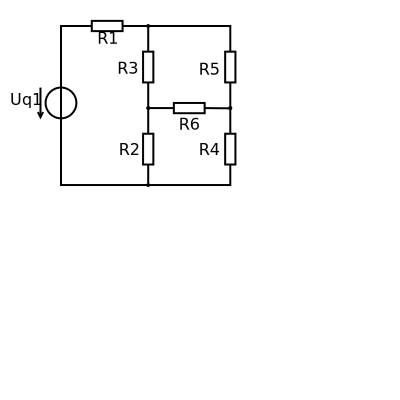
\includegraphics{messbruecke1}
    \caption{Messbrücke}}
    \only<2>{\includegraphics{messbruecke1_1}
    \caption{Messbrücke mit vollständigem Baum} }
    \only<3>{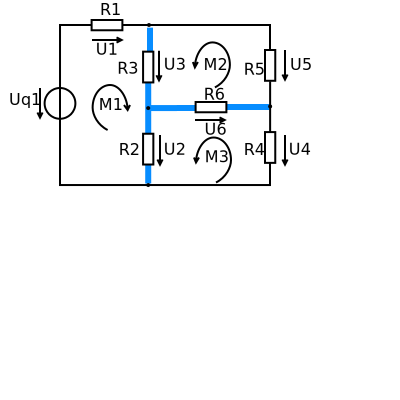
\includegraphics{messbruecke1_2}
    \caption{Messbrücke mit vollständigem Baum und Maschen} }
    \label{abb:Messbruecke1}
  \end{figure}
\end{frame}

\begin{figure}[htbp]
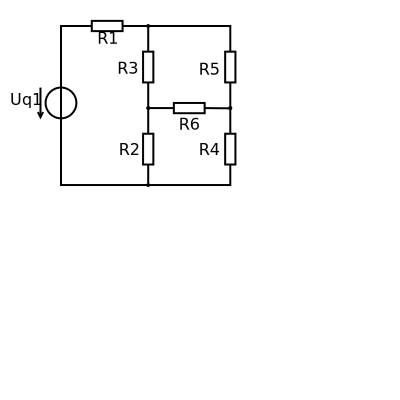
\includegraphics{messbruecke1}
    \caption{Messbrücke}
\end{figure}

Im ersten Schritt muss ein sogenannter Baum festgelegt werden. Der Baum muss alle Knoten verbinden, darf aber keinen geschlossenen Umlauf bilden.

\begin{figure}[htbp]
 \includegraphics{messbruecke1_1}
 \caption{Messbrücke mit vollständigem Baum}
 \label{abb:Messbruecke1_Baum}
\end{figure}

Die Maschen M1, M2 und M3 bestehen immer aus einer Sehne (ein Zweig, der nicht zum vollständigen Baum gehört) und Zweigen, die zum Baum gehören.

Für das Gleichungssystem ist die Umlaufrichtung der Maschen relevant. M1 dreht im Uhrzeigersinn, da hier die Quelle Uq1 in der Masche ist. Der Spannungspfeil der Quelle sollte möglichst gegen die Umlaufrichtung der Masche gerichtet sein.

\begin{figure}[htbp]
  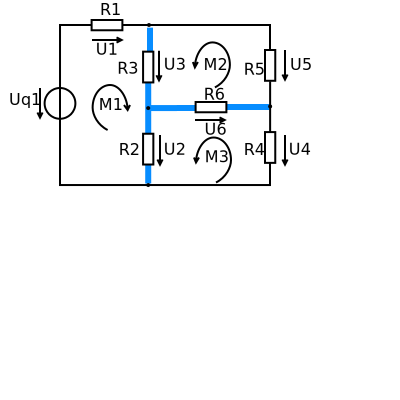
\includegraphics{messbruecke1_2}
  \caption{Messbrücke mit vollständigem Baum und Maschen}
\end{figure}

Im nächsten Schritt stelle ich für alle Maschen und alle Knoten Gleichungen auf.


\begin{align}
 M1: & -Uq1 + U1 + U3 + U2 = 0\\
 M2: & U3 + U6 - U5 = 0 \\
 M3: & U2 - U6 - U4 = 0\\
\end{align}

\begin{frame}<presentation>
  \frametitle{Gleichungen für Maschen und Knoten}

\begin{align}
 M1: & -Uq1 + U1 + U3 + U2 = 0\\
 M2: & U3 + U6 - U5 = 0 \\
 M3: & U2 - U6 - U4 = 0\\
\end{align}

Knotengleichungen:\\
\begin{align}
  \text{I:}\ & I1 - I3 - I5 = 0\\
  \text{II:}\ & I3 - I2 - I6 = 0\\
  \text{III:}\ & I2 + I4 -I1 = 0
\end{align}
\end{frame}



Für die Knoten gilt, dass die Summer aller Ströme, die hinein fließen und die Summe aller Ströme, die hinaus fließen null sein muss. $\sum_{k=1}^n I_k = 0$

Knotengleichungen:\\
\begin{align}
  \text{I:}\ & I1 - I3 - I5 = 0\\
  \text{II:}\ & I3 - I2 - I6 = 0\\
  \text{III:}\ & I2 + I4 -I1 = 0
\end{align}

Die Ströme seien gleich der Spannungspfeile an den Widerständen.
Ich zähle Ströme, die in den Knoten hinein fließen positiv, Ströme, die aus dem Knoten heraus fließen negativ.

Zur Berechnung der Ströme und Spannungen kann ich die Gleichungen der Maschen und der Knoten zu einem linearen Gleichungssystem (LGS) zusammenfassen. Wichtig dabei ist, dass das Gleichungssystem nicht über bestimmt ist. Es dürfen nur die Gleichungen in das System übernommen werden, die linear unabhängig sind. Z. B. alle Maschengleichungen oder alle Knotengleichungen. Eine Kombination aus Maschengleichungen und Knotengleichungen ist auch möglich, solange alle Gleichungen des LGS linear unabhängig sind.

Mit Hilfe der Maschengleichungen und Widerstände in den Zweigen kann ich die Ströme in den Zweigen bestimmen:

\begin{frame}{Berechnung der Ströme}
\begin{align}
-Uq1 + I1 * R1 + I3 * R3 + I2 * R2 &= 0\\
I3 * R3 + I6 * R6 - I5 * R5 &= 0 \\
I2 * R2 - I6 * R6 - I4 * R4 &= 0
\end{align}
\end{frame}

Das LGS ist dabei in eine Stufenform zu überführen. Zur leichteren Berechnung verwende ich die Matrix-Schreibweise:

\begin{frame}{LGS aufstellen}
$\left( \begin{array}{rrrrrr}
    1 &     0  & -1     &     0 & -1    &     0\\
    0 & -1     & 1      &     0 &   0   &     0\\
  -1  & 1      &   0    & 1     & 0     & 0    \\
R1 & R2 & R3 & 0  & 0  & 0\\
0  & 0  & R3 & 0  & R5 & R6 \\
0  & R2 & 0  & R4 & 0  & R6 \\
\end{array}\right) *
\left(\begin{array}{c}
       I1\\
       I2\\
       I3\\
       I4\\
       I5\\
       I6
      \end{array} \right)
= \left( \begin{array}{c}
  0\\
  0\\
  0\\
  Uq1\\
  0\\
  0
 \end{array}\right)
$
\end{frame}

Für die Berechnung werden die Elemente der Matrix links (Widerstände) mit den Elementen des Spalten-Vektors (Ströme) einzeln multipliziert und anschließend addiert.

$\begin{array}{lllllll}
    1 &     0  & -1     &     0 & -1    &     0 &= 0\\
    0 & -1     & 1      &     0 &   0   &     0 &= 0\\
  -1  & 1      &   0    & 1     & 0     & 0     &= 0\\
R1*I1 &+ R2*I2 &+ R3*I3 &+ 0*I4 &+ 0*I5 &+0*I6  &= Uq1\\
0*I1  &+0*I2   &+R3*I3  &+0*I4  &+R5*I5 &+R6*I6 &= 0\\
0*I1  &+ R2*I2 &+0*I3   &+R4*I4 &+0*I5  &+R6*I6 &= 0
\end{array}$

Überführung in die Stufenform. \\Im ersten Schritt vertausche ich Zeile fünf und sechs der Widerstands-Matrix und des Ergebnis-Vektors. Der Vektor mit den Strömen bleibt gleich.

$\left( \begin{array}{rrrrrr}
    1 &     0  & -1     &     0 & -1    &     0\\
    0 & -1     & 1      &     0 &   0   &     0\\
  -1  & 1      &   0    & 1     & 0     & 0    \\
R1 & R2 & R3 & 0  & 0  & 0\\
0  & R2 & 0  & R4 & 0  & R6 \\
0  & 0  & R3 & 0  & R5 & R6 \\
\end{array}\right) *
\left(\begin{array}{c}
       I1\\
       I2\\
       I3\\
       I4\\
       I5\\
       I6
      \end{array} \right)
= \left( \begin{array}{c}
 0\\
 0\\
 0\\
 Uq1\\
 0\\
 0
 \end{array}\right)
$

Oft schreibt man die verkürzte Darstellung. Der Vektor mit Strömen wird in diesem Fall nicht dargestellt, Der Vektor mit den Spannungen wird durch eine senkrechte Linie vom Array der Widerstände bzw. Vorfaktoren der Ströme abgetrennt.

\begin{frame}{Gekürzte Darstellung der Matrix}

$\left( \begin{array}{rrrrrr|r}
 1 &  0 & -1 & 0  & -1 &  0 & 0\\
 0 & -1 &  1 & 0  &  0 &  0 & 0\\
-1 &  1 &  0 & 1  &  0 &  0 & 0 \\
R1 & R2 & R3 & 0  &  0 &  0 & Uq1\\
0  & R2 & 0  & R4 &  0 & R6 & 0 \\
0  & 0  & R3 & 0  & R5 & R6 & 0\\
\end{array}\right)
$
\end{frame}

Mit dem gaußschen Eliminationsverfahren kann ich die Matrix (links der senkrechten Linie) in eine Dreiecks-Form bringen. Dazu kann ich jeweils zwei Zeilen vertauschen oder durch Multiplikation von Faktoren zwei Zeilen addieren, sodass in einzelnen Spalten 0-Werte gebildet werden. Ziel der Umrechnung ist, dass die Matrix etwa die Form

\begin{frame}{Stufenform - Beispiel}
$\left( \begin{array}{rrr}
 1 & 2 & 3 \\
 0 & 3 & 2 \\
 0 & 0 & 3
\end{array}\right)$
\end{frame}

erreicht. Das gaußsche Eliminationsverfahren stelle ich an dieser Stelle nicht vertieft dar. Bei Wikipedia ist ein ausführlicher Artikel zum Algorithmus des Verfahrens zu finden.

Wen ich die Matrix in die Dreiecks-Form überführt habe, kann ich von unten nach oben die Werte einsetzen und die Ströme berechnen. Da diese Vorgehen aufwändig und fehleranfällig ist, kann man alternativ die Verfahren der Maschenanalyse (Kreisstromverfahren) oder die Knotenanalyse (Knotenspannungsverfahren oder Knotenpotentialverfahren) verwenden.
\clearpage

\section[noch offen]{Pflicht-Themen, die noch offen sind}
\begin{frame}{Pflicht-Themen, die noch offen sind}
  Folgende Themen sind gemäß Prüfungserlass für die Prüfung 2026 Pflicht, aber noch nicht ausgearbeitet.
  \begin{itemize}
%         \item Knoten- und Maschengleichungen
    \item Kreisstromverfahren
    \item Knotenspannungsverfahren
  \end{itemize}

  Die Themen folgen demnächst hier.
\end{frame}


    % \section[Kreisstrom]{Kreisstromverfahren (Pflicht)}
    % \begin{frame}<beamer>
    %   \frametitle{Inhalt}
    %   \tableofcontents[currentsection, hideothersubsections]
    % \end{frame}


    % \section[Knotenspannung]{Knotenspannungsverfahren (Pflicht)}
    % \begin{frame}<beamer>
    %   \frametitle{Inhalt}
    %   \tableofcontents[currentsection, hideothersubsections]
    % \end{frame}

    %%%%%%%%%%%%%%%%%%%%%%%%%%%%%%%%%%
    %   \section{Maschenstromanalyse}
    %
    %
    %   $\begin{vmatrix}
    %     1 & 0 & 0 \\
    %     0 & 1 & 0 \\
    %     0 & 0 & 1 \\
    %   \end{vmatrix}$
    %   \\
    %   $\begin{array}{|rr|r|}
    %     1 & 0 & 0 \\
    %     0 & 1 & 0 \\
    %     0 & 0 & 1 \\
    %   \end{array}$
    %   \section{Knotenpotentialanalyse}

    \section{Lösungen}
    \subsection{Ersatzwiderstand}
    \label{lsg:Ersatzwiderstand}
    \subsubsection{Übungen zu Zweipole I}
    \begin{description}
      \item[a] $R1 = R2 = 220 \Omega \ R3 = R5 = 230 \Omega \ R4 = 470 \Omega$ \ $R{3||45} = 173,12 \Omega$
      \item[b] $R1 = R2 = R3 = R5 = 230 \Omega \ R4 = 560 \Omega$ \ $R{3||45} = 178,14 \Omega$
      \item[c] $R1 = R2 = R4 = R5 = 150 \Omega \ R3 = 120 \Omega$ \ $R{3||45} = 85,71 \Omega$
    \end{description}
    \subsubsection{Übungen zu Zweipole II}
    \begin{description}
      \item[a] $R1 = R2 = 220 \Omega \ R3 = R5 = 230 \Omega \ R4 = 470 \Omega$ \ $R_{3||5+4} = 585,01 \Omega$
      \item[b] $R1 = R2 = R3 = 150 \Omega \ R5 = 230 \Omega \ R4 = 560 \Omega$ \ $R_{3||5+4} =  650,79\Omega$
      \item[c] $R1 = R2 = R4 = R5 = 150 \Omega \ R3 = 120 \Omega$ \ $R_{3||5+4} =  216,67\Omega$
    \end{description}


    \subsection{Spannungsteiler}
    \label{Lsg:Spannungsteiler}
    Zu Aufgabe aus Abschnitt \ref{Aufg:Spannungsteiler}

    \begin{tabular}{l|ll|ll}
      U [V] & $R_1 [\Omega]$& $R_2 [\Omega]$& $I_{R1}$ & $I_{R2}$\\ \hline
      5     & 220 & 330  & 9,09 mA  & 9,09 mA  \\
      12    & 220 & 470  & 17,39 mA & 17,39 mA \\
      12    & 220 & 780  & 12 mA    & 12 mA    \\
      12    & 470 & 683  & 10,4 mA  & 10,4 mA  \\
      14,96 & 560 & 120  & 22 mA    & 22 mA    \\
      6,5   & 470 & 1,5k &  3,3 mA  &  3,3 mA  \\
    \end{tabular}
    \subsection{Lösungsvorschlag zu Schaltung 2}
    %   Die Bilder für Schaltung 2 und Schaltung 3 sind hier zurzeit überlagert. In der Beamer-Version sind die Bilder gut erkennbar.
    \begin{frame}<article=0>
      \frametitle{Schaltung 2- nur Quelle 1 aktiv}
      \begin{columns}
        \begin{column}{.6\textwidth}
          \begin{figure}[htb]
            \begin{circuitikz}
              \draw (0,0) to [vsource, l=$U_{q1}$] (0,4);
              \draw (0,4) to [R=$R_1$] (2,4) node[circ]{} node[above]{A} to [R=$R_2$] (2,2.5) to [short, i>_=$I_2$]  (2,2) ;
              \draw (2,2) to [R=$R_3$,  v=$U_3$, voltage=straight] (2,0) node[circ]{} node[below]{B}  -- (0,0);
              \only<1-3>{\draw (2,2) node[circ]{} -- (3,2) -- (4,2) to[short] (4,2)  to[R=$R_4$] (4,0);}
              \draw (4,0) -- (2,0);
              \only<1-2>{ \draw (2,4) -- (4,4) to [R=$R_5$] (6,4);}
              \only<1-2>{\draw (6,4) to [R=$R_6$] (6,2);}
              \only<3->{\draw (6,4) to [R=$R_{5+6}$] (6,2);
                \draw (2,4) -- (6,4);}
              \draw (6,2) -- (6,0) -- (6,0);
              \only<4>{\draw (2,2) to [R=$R_{3||4}$,  v=$U_3$, voltage=straight] (2,0);}
              \only<1-3>{\draw (6,0) to [short, -*] (4,0);}
              \only<4>{\draw (6,0) -- (4,0);}
              \only<2>{\draw[red, thick] (4,2.3) rectangle
                (6.8,4.8);}
              \only<3>{\draw[red, thick] (1.3,-0.5) rectangle
                (4.8,2.3);}
            \end{circuitikz}
            \caption{Überlagerung, Schaltung 2}
            \label{fig:SchaltungZweiLsgVorschlagTeil1}
          \end{figure}
        \end{column}
        \begin{column}{.4\textwidth}
          $R1 = 100\Omega ,\ R2 = 220 \Omega$ $R3 = 270\Omega ,\ R4 = 470 \Omega$ $R5 = 560 \Omega,\ R6 = 180 \Omega$ $U_{q1} = 12\,V, U_{q2} = 15\,V$
        \end{column}
      \end{columns}
    \end{frame}

    Gegeben seien die Werte: $R1 = 100\Omega ,\ R2 = 220 \Omega$ $R3 = 270\Omega ,\ R4 = 470 \Omega$ $R5 = 560 \Omega,\ R6 = 180 \Omega$ $U_{q1} = 12\,V, U_{q2} = 15\,V$

    Da ich die Spannung an R3 berechnen soll, kann ich die Schaltung nur bis Bild \ref{fig:SchaltungZweiLsgVorschlagTeil1_14} / \ref{fig:SchaltungZweiLsgVorschlagTeil2_24} zusammenfassen.

    \subsubsection{Schaltung 2 - nur Quelle 1 aktiv}
    \begin{figure}[htbp]
      \begin{circuitikz}
        \draw (0,0) to [vsource, l=$U_{q1}$] (0,4);
        \draw (0,4) to [R=$R_1$] (2,4) node[circ]{} node[above]{A} to [R=$R_2$] (2,2.5) to [short, i>_=$I_2$]  (2,2) ;
        \draw (2,2) to [R=$R_3$,  v=$U_3$, voltage=straight] (2,0) node[circ]{} node[below]{B}  -- (0,0);
        \only<1-3>{\draw (2,2) node[circ]{} -- (3,2) -- (4,2) to[short] (4,2)  to[R=$R_4$] (4,0);}
        \draw (4,0) -- (2,0);
        \only<1-2>{ \draw (2,4) -- (4,4) to [R=$R_5$] (6,4);}
        \only<1-2>{\draw (6,4) to [R=$R_6$] (6,2);}
        \draw (6,2) -- (6,0) -- (6,0);
        \only<1-3>{\draw (6,0) to [short, -*] (4,0);}
      \end{circuitikz}
      \caption{Überlagerung, Schaltung 2 (Schritt 1.1)}
      \label{fig:SchaltungZweiLsgVorschlagTeil1_11}
    \end{figure}

    \begin{figure}[htbp]
      \begin{circuitikz}
        \draw (0,0) to [vsource, l=$U_{q1}$] (0,4);
        \draw (0,4) to [R=$R_1$] (2,4) node[circ]{} node[above]{A} to [R=$R_2$] (2,2.5) to [short, i>_=$I_2$]  (2,2) ;
        \draw (2,2) to [R=$R_3$, v=$U_3$, voltage=straight] (2,0) node[circ]{} node[below]{B} -- (0,0);
        \draw (2,2) node[circ]{} -- (3,2) -- (4,2) to[short] (4,2) to[R=$R_4$] (4,0);
        \draw (4,0) -- (2,0);
        \draw (2,4) -- (4,4) to [R=$R_5$] (6,4);
        \draw (6,4) to [R=$R_6$] (6,2);
        \draw (2,4) -- (6,4);
        \draw (6,2) -- (6,0) -- (6,0);
        \draw (6,0) to [short, -*] (4,0);
        \draw[red, thick] (4,2.3) rectangle
        (6.8,4.8);
      \end{circuitikz}
      \caption{Überlagerung, Schaltung 2 (Schritt 1.2)}
      \label{fig:SchaltungZweiLsgVorschlagTeil1_12}
    \end{figure}


    \begin{figure}[htbp]
      \begin{circuitikz}
        \draw (0,0) to [vsource, l=$U_{q1}$] (0,4);
        \draw (0,4) to [R=$R_1$] (2,4) node[circ]{} node[above]{A} to [R=$R_2$] (2,2.5) to [short, i>_=$I_2$]  (2,2) ;
        \draw (2,2) to [R=$R_3$, v=$U_3$, voltage=straight] (2,0) node[circ]{} node[below]{B} -- (0,0);
        \draw (2,2) node[circ]{} -- (3,2) -- (4,2) to[short] (4,2) to[R=$R_4$] (4,0);
        \draw (4,0) -- (2,0);
        \draw (6,4) to [R=$R_{5+6}$] (6,2);
        \draw (2,4) -- (6,4);
        \draw (6,2) -- (6,0) -- (6,0);
        %     \only<4>{\draw (2,2) to [R=$R_{3||4}$, v=$U_3$] (2,0);}
        \draw (6,0) to [short, -*] (4,0);
        %     \only<4>{\draw (6,0) -- (4,0);}
        \draw[red, thick] (1.3,-0.5) rectangle
        (4.8,2.3);
      \end{circuitikz}
      \caption{Überlagerung, Schaltung 2 (Schritt 1.3)}
      \label{fig:SchaltungZweiLsgVorschlagTeil1_13}
    \end{figure}

    \begin{figure}[ht]
      \begin{circuitikz}
        \draw (0,0) to [vsource, l=$U_{q1}$] (0,4);
        \draw (0,4) to [R=$R_1$] (2,4) node[circ]{} node[above]{A} to [R=$R_2$] (2,2.5) to [short, i>_=$I_2$] (2,2) ;
        \draw (2,2) to [R=$R_3$,  v=$U_3$, voltage=straight] (2,0) node[circ]{} node[below]{B} -- (0,0);
        \draw (4,0) -- (2,0);
        \draw (6,4) to [R=$R_{5+6}$] (6,2);
        \draw (2,4) -- (6,4);
        \draw (6,2) -- (6,0) -- (6,0);
        \draw (2,2) to [R=$R_{3||4}$, v=$U_3$, voltage=straight] (2,0);
        \draw (6,0) -- (4,0);
      \end{circuitikz}
      \caption{Überlagerung, Schaltung 2 (Schritt 1.4)}
      \label{fig:SchaltungZweiLsgVorschlagTeil1_14}
    \end{figure}

    \clearpage
    \subsubsection{Schaltung 2 - nur Quelle 2 aktiv}
    \begin{frame}<article=0>{Schaltung 2- nur Quelle 2 aktiv}
      \begin{columns}
        \begin{column}{.6\textwidth}
          \begin{figure}[htbp]
            \begin{circuitikz}
              \draw (6,1.5) to [vsource, l=$U_{q2}$] (6,0) -- (6,0);
              \draw (0,4) -- (0,0);
              \draw (0,4) to [R=$R_1$] (2,4) node[circ]{} node[above]{A} to [R=$R_2$] (2,2.5) to [short, i>_=$I_2$] (2,2) ;
              \draw (2,2) to [R=$R_3$, v=$U_3$, voltage=straight] (2,0) node[circ]{} node[below]{B} -- (0,0);
              \only<1-3>{\draw (2,2) node[circ]{} -- (3,2) -- (4,2) to[short] (4,2) to[R=$R_4$] (4,0);}
              \draw (4,0) -- (2,0);
              \only<1-2>{ \draw (2,4) -- (4,4) to [R=$R_5$] (6,4);}
              \only<1-2>{\draw (6,4) to [R=$R_6$] (6,2);}
              \only<3->{\draw (6,4) to [R=$R_{5+6}$] (6,2);
                \draw (2,4) -- (6,4);}
              \draw (6,2) -- (6,0) -- (6,0);
              \only<4>{\draw (2,2) to [R=$R_{3||4}$,  v=$U_3$, voltage=straight] (2,0);}
              \only<1-3>{\draw (6,0) to [short, -*] (4,0);}
              \only<4>{\draw (6,0) -- (4,0);}
              \only<2>{\draw[red, thick] (4,2.3) rectangle
                (6.8,4.8);}
              \only<3>{\draw[red, thick] (1.3,-0.5) rectangle
                (4.8,2.3);}
            \end{circuitikz}
            \caption{Überlagerung, Schaltung 2}
            \label{fig:SchaltungZweiLsgVorschlagTeil2}
          \end{figure}
        \end{column}
        \begin{column}{.4\textwidth}
          $R1 = 100\Omega ,\ R2 = 220 \Omega$ $R3 = 270\Omega ,\ R4 = 470 \Omega$ $R5 = 560 \Omega,\ R6 = 180 \Omega$ $U_{q1} = 12\,V, U_{q2} = 15\,V$
        \end{column}
      \end{columns}
    \end{frame}

    \begin{figure}[hb]
      \begin{circuitikz}
        \draw (6,1.5) to [vsource, l=$U_{q2}$] (6,0) -- (6,0);
        \draw (0,4) -- (0,0);
        \draw (0,4) to [R=$R_1$] (2,4) node[circ]{} node[above]{A} to [R=$R_2$] (2,2.5) to [short, i>_=$I_2$] (2,2) ;
        \draw (2,2) to [R=$R_3$, v=$U_3$, voltage=straight] (2,0) node[circ]{} node[below]{B} -- (0,0);
        \draw (2,2) node[circ]{} -- (3,2) -- (4,2) to[short] (4,2) to[R=$R_4$] (4,0);
        \draw (4,0) -- (2,0);
        \draw (2,4) -- (4,4) to [R=$R_5$] (6,4);
        \draw (6,4) to [R=$R_6$] (6,2);
        \draw (6,2) -- (6,0) -- (6,0);
        \draw (6,0) to [short, -*] (4,0);
      \end{circuitikz}
      \caption{Überlagerung, Schaltung 2 (Schritt 2.1)}
      \label{fig:SchaltungZweiLsgVorschlagTeil2_21}
    \end{figure}

    $R1 = 100\Omega ,\ R2 = 220 \Omega$ $R3 = 270\Omega ,\ R4 = 470 \Omega$ $R5 = 560 \Omega,\ R6 = 180 \Omega$ $U_{q1} = 12\,V, U_{q2} = 15\,V$

    \begin{figure}[htbp]
      \begin{circuitikz}
        \draw (6,1.5) to [vsource, l=$U_{q2}$] (6,0) -- (6,0);
        \draw (0,4) -- (0,0);
        \draw (0,4) to [R=$R_1$] (2,4) node[circ]{} node[above]{A} to [R=$R_2$] (2,2.5) to [short, i>_=$I_2$] (2,2) ;
        \draw (2,2) to [R=$R_3$, v=$U_3$, voltage=straight] (2,0) node[circ]{} node[below]{B} -- (0,0);
        \draw (2,2) node[circ]{} -- (3,2) -- (4,2) to[short] (4,2) to[R=$R_4$] (4,0);
        \draw (4,0) -- (2,0);
        \draw (2,4) -- (4,4) to [R=$R_5$] (6,4);
        \draw (6,4) to [R=$R_6$] (6,2);
        \draw (6,2) -- (6,0) -- (6,0);
        \draw (6,0) to [short, -*] (4,0);
        \draw[red, thick] (4,2.3) rectangle
        (6.8,4.8);
      \end{circuitikz}
      \caption{Überlagerung, Schaltung 2 (Schritt 2.2)}
      \label{fig:SchaltungZweiLsgVorschlagTeil2_22}
    \end{figure}

    \begin{figure}[htbp]
      \begin{circuitikz}
        \draw (6,1.5) to [vsource, l=$U_{q2}$] (6,0) -- (6,0);
        \draw (0,4) -- (0,0);
        \draw (0,4) to [R=$R_1$] (2,4) node[circ]{} node[above]{A} to [R=$R_2$] (2,2.5) to [short, i>_=$I_2$] (2,2) ;
        \draw (2,2) to [R=$R_3$, v=$U_3$, voltage=straight] (2,0) node[circ]{} node[below]{B} -- (0,0);
        \draw (2,2) node[circ]{} -- (3,2) -- (4,2) to[short] (4,2) to[R=$R_4$] (4,0);
        \draw (4,0) -- (2,0);
        \draw (6,4) to [R=$R_{5+6}$] (6,2);
        \draw (2,4) -- (6,4);
        \draw (6,2) -- (6,0) -- (6,0);
        \draw (6,0) to [short, -*] (4,0);
        \draw[red, thick] (1.3,-0.5) rectangle
        (4.8,2.3);
      \end{circuitikz}
      \caption{Überlagerung, Schaltung 2 (Schritt 2.3)}
      \label{fig:SchaltungZweiLsgVorschlagTeil2_23}
    \end{figure}

    \begin{figure}[htbp]
      \begin{circuitikz}
        \draw (6,1.5) to [vsource, l=$U_{q2}$] (6,0) -- (6,0);
        \draw (0,4) -- (0,0);
        \draw (0,4) to [R=$R_1$] (2,4) node[circ]{} node[above]{A} to [R=$R_2$] (2,2.5) to [short, i>_=$I_2$] (2,2) ;
        \draw (2,2) to [R=$R_3$, v=$U_3$, voltage=straight] (2,0) node[circ]{} node[below]{B} -- (0,0);
        \only<1-3>{\draw (2,2) node[circ]{} -- (3,2) -- (4,2) to[short] (4,2) to[R=$R_4$] (4,0);}
        \draw (4,0) -- (2,0);
        \draw (6,4) to [R=$R_{5+6}$] (6,2);
        \draw (2,4) -- (6,4);
        \draw (6,2) -- (6,0) -- (6,0);
        \draw (2,2) to [R=$R_{3||4}$, v=$U_3$, voltage=straight] (2,0);
        \draw (6,0) -- (4,0);
      \end{circuitikz}
      \caption{Überlagerung, Schaltung 2 (Schritt 2.4)}
      \label{fig:SchaltungZweiLsgVorschlagTeil2_24}
    \end{figure}

    \clearpage
    \subsection{Lösungsvorschlag zu Schaltung 3}
    \subsubsection{Schaltung 3 - nur Quelle 1 aktiv}

    \begin{frame}<article=0>{Schaltung 3 - nur Quelle 1 aktiv}
      \begin{columns}
        \begin{column}{.6\textwidth}
          \begin{figure}[htbp]
            \begin{circuitikz}
              \draw (0,0) to [vsource, l=$U_{q1}$] (0,4);
              \draw (0,4) to [R=$R_1$] (2,4) node[circ]{} node[above]{A} to (2,2);
              \only<1-3>{\draw (2,2) node[left]{B} to [short, i>_=$I_4$] (2,1.5);}
              \only<4->{\draw (2,1.5) -- (2,2);}% node[circ]{} -- (4,2);}
              \draw (2,1.5)to [R=$R_{4||6}$,  v=$U_4$, voltage=straight] (2,0) node[circ]{} node[below]{GND} -- (0,0);
              \only<1-4>{\draw (2,4) to [R=$R_2$] (4,4);}
              \only<5->{\draw (2,4) -- (4,4) to [R=$R_{(2||5)+3+7}$] (4,0);}
              \only<1-3>{\draw (4,4) node[circ]{} node[above]{C} to [R=$R_5$] (4,2);}
              \only<4>{\draw (4,4) node[circ]{} node[above]{C} -- (4,3)
                to [R=$R_5$] (2,3) node[circ]{};}
              \only<1-3>{\draw (2,2) node[circ]{} -- (4,2)};
              \only<1-3>{\draw (4,2) node[circ]{} node[right]{D} -- (4,2) to[R=$R_6$] (4,0) -- (3,0) -- (2,0);}
              \only<4->{\draw (4,0) -- (3,0) -- (2,0);}
              \only<1-2>{\draw (4,4) to [R=$R_3$] (6,4);
                \draw (6,4) to [R=$R_7$] (6,2);}
              \only<3-4>{\draw (4,4) -- (6,4) to [R=$R_{3+7}$] (6,2);}
              %\draw (6,2) to [vsource, l=$U_{q2}$] (6,0);
              \only<1-4>{\draw (6,2) -- (6,0);}
              \only<1-3>{\draw (6,0) to [short, -*] (4,0);}
              \only<4>{\draw (6,0) -- (4,0);}
              \only<2>{\draw[red, thick] (4.3,2.3) rectangle
                (6.8,4.8);}
              \only<3>{\draw[red, thick] (1.3,-0.5) rectangle
                (4.8,2.3);}
            \end{circuitikz}
            \caption{Überlagerung, Schaltung 3}
            \label{fig:SchaltungDreiLsgVorschlagTeil1}
          \end{figure}
        \end{column}
        \begin{column}{.4\textwidth}
          $R1 = 100\Omega ,\ R2 = 220 \Omega$ $R3 = 270\Omega ,\ R4 = 470 \Omega $ $ R5 = 470 \Omega,\ R6 = 560\Omega$
          $ R7 = 120 \Omega$
          $U_{q1} = 12\,V, U_{q2} = 15\,V$
        \end{column}
      \end{columns}
    \end{frame}

    $R1 = 100\Omega ,\ R2 = 220 \Omega$ $R3 = 270\Omega ,\ R4 = 470 \Omega $ $ R5 = 470 \Omega,\ R6 = 560\Omega$
    $ R7 = 120 \Omega$
    $U_{q1} = 12\,V, U_{q2} = 15\,V$


    \begin{figure}[htbp]
      \begin{circuitikz}
        \draw (0,0) to [vsource, l=$U_{q1}$] (0,4);
        \draw (0,4) to [R=$R_1$] (2,4) node[circ]{} node[above]{A} to (2,2);
        \only<1-3>{\draw (2,2) node[left]{B} to [short, i>_=$I_4$] (2,1.5);}
        \draw (2,1.5)to [R=$R_{4}$, v=$U_4$, voltage=straight] (2,0) node[circ]{} node[below]{GND} -- (0,0);
        \draw (2,4) to [R=$R_2$] (4,4);
        \draw (4,4) node[circ]{} node[above]{C} to [R=$R_5$] (4,2);
        \draw (2,2) node[circ]{} -- (4,2);
        \draw (4,2) node[circ]{} node[right]{D} -- (4,2) to[R=$R_6$] (4,0) -- (3,0) -- (2,0);
        \draw (4,4) to [R=$R_3$] (6,4);
        \draw (6,4) to [R=$R_7$] (6,2);
        \draw (6,2) -- (6,0);
        \draw (6,0) to [short, -*] (4,0);
      \end{circuitikz}
      \caption{Überlagerung, Schaltung 3, (Schritt1.1) Quelle Q2 entfernt}
      \label{fig:SchaltungDreiLsgVorschlagTeil11}
    \end{figure}

    \begin{figure}[htbp]
      \begin{circuitikz}
        \draw (0,0) to [vsource, l=$U_{q1}$] (0,4);
        \draw (0,4) to [R=$R_1$] (2,4) node[circ]{} node[above]{A} to (2,2);
        \draw (2,2) node[left]{B} to [short, i>_=$I_4$] (2,1.5);
        \draw (2,1.5)to [R=$R_{4||6}$, v=$U_4$, voltage=straight] (2,0) node[circ]{} node[below]{GND} -- (0,0);
        \draw (2,4) to [R=$R_2$] (4,4);
        \draw (4,4) node[circ]{} node[above]{C} to [R=$R_5$] (4,2);
        \draw (2,2) node[circ]{} -- (4,2);
        \draw  (4,0) -- (3,0) -- (2,0);
        \draw (4,4) -- (6,4) to [R=$R_{3+7}$] (6,2);
        \draw (6,2) -- (6,0);
        \draw (6,0) -- (4,0);
      \end{circuitikz}
      \caption{Überlagerung, Schaltung 3, (Schritt1.2)}
      \label{fig:SchaltungDreiLsgVorschlagTeil12}
    \end{figure}

    \begin{figure}[htbp]
      \begin{circuitikz}
        \draw (0,0) to [vsource, l=$U_{q1}$] (0,4);
        \draw (0,4) to [R=$R_1$] (2,4) node[circ]{} node[above]{A} to (2,2);
        \draw (2,1.5) -- (2,2);
        \draw (2,1.5)to [R=$R_{4||6}$, v=$U_4$, voltage=straight] (2,0) node[circ]{} node[below]{GND} -- (0,0);
        \draw (2,4) to [R=$R_2$] (4,4);
        \draw (4,4) node[circ]{} node[above]{C} -- (4,3)
        to [R=$R_5$] (2,3) node[circ]{};
        \draw (4,0) -- (3,0) -- (2,0);

        \draw (4,4) -- (6,4) to [R=$R_{3+7}$] (6,2);
        \draw (6,2) to [vsource, l=$U_{q2}$] (6,0);
        \draw (6,2) -- (6,0);
        \draw (6,0) -- (4,0);
      \end{circuitikz}
      \caption{Überlagerung, Schaltung 3, (Schritt1.4)}
      \label{fig:SchaltungDreiLsgVorschlagTeil14}
    \end{figure}

    \begin{figure}[htbp]
      \begin{circuitikz}
        \draw (0,0) to [vsource, l=$U_{q1}$] (0,4);
        \draw (0,4) to [R=$R_1$] (2,4) node[circ]{} node[above]{A} to (2,2);
        \draw (2,2)to [R=$R_{4||6}$, v=$U_4$, voltage=straight] (2,0) node[circ]{} node[below]{GND} -- (0,0);
        \draw (2,4) -- (4,4) to [R=$R_{(2||5)+3+7}$] (4,0);
        \draw (4,0) -- (3,0) -- (2,0);
      \end{circuitikz}
      \caption{Überlagerung, Schaltung 3, (Schritt1.5)}
      \label{fig:SchaltungDreiLsgVorschlagTeil15}
    \end{figure}

    \begin{frame}<article=0>{Schaltung 3 - nur Quelle 2 aktiv}
      \begin{columns}
        \begin{column}{.6\textwidth}
          \begin{figure}[htbp]
            \begin{circuitikz}
              %             \draw (0,0) to [vsource, l=$U_{q1}$] (0,4);
              \draw (0,4) -- (0,0);
              \draw (0,4) to [R=$R_1$] (2,4) node[circ]{} node[above]{A} to (2,2);
              \only<1-3>{\draw (2,2) node[left]{B} to [short, i>_=$I_4$] (2,1.5);}
              \only<4->{\draw (2,1.5) -- (2,2);}% node[circ]{} -- (4,2);}
              \draw (2,1.5)to [R=$R_{4||6}$, v=$U_4$, voltage=straight] (2,0) node[circ]{} node[below]{GND} -- (0,0);
              \only<1-4>{\draw (2,4) to [R=$R_2$] (4,4);}
              \only<5->{\draw (2,4) -- (6,4) to [R=$R_{(2||5)+3+7}$] (6,2);}
              \only<1-3>{\draw (4,4) node[circ]{} node[above]{C} to [R=$R_5$] (4,2);}
              \only<4>{\draw (4,4) node[circ]{} node[above]{C} -- (4,3)
                to [R=$R_5$] (2,3) node[circ]{};}
              \only<1-3>{\draw (2,2) node[circ]{} -- (4,2)};
              \only<1-3>{\draw (4,2) node[circ]{} node[right]{D} -- (4,2) to[R=$R_6$] (4,0) -- (3,0) -- (2,0);}
              \only<4->{\draw (4,0) -- (3,0) -- (2,0);}
              \only<1-2>{\draw (4,4) to [R=$R_3$] (6,4);
                \draw (6,4) to [R=$R_7$] (6,2);}
              \only<3-4>{\draw (4,4) -- (6,4) to [R=$R_{3+7}$] (6,2);}
              \draw (6,2) to [vsource, l=$U_{q2}$] (6,0);
              \only<1-4>{\draw (6,2) -- (6,0);}
              \only<1-3>{\draw (6,0) to [short, -*] (4,0);}
              \only<4->{\draw (6,0) -- (4,0);}
              \only<2>{\draw[red, thick] (4.3,2.3) rectangle
                (6.8,4.8);}
              \only<3>{\draw[red, thick] (1.3,-0.5) rectangle
                (4.8,2.3);}
            \end{circuitikz}
            \caption{Überlagerung, Schaltung 3}
            \label{fig:SchaltungDreiLsgVorschlagTeil2}
          \end{figure}
        \end{column}
        \begin{column}{.4\textwidth}
          $R1 = 100\Omega ,\ R2 = 220 \Omega$ $R3 = 270\Omega ,\ R4 = 470 \Omega $ $ R5 = 470 \Omega,\ R6 = 560\Omega$
          $ R7 = 120 \Omega$
          $U_{q1} = 12\,V, U_{q2} = 15\,V$
        \end{column}
      \end{columns}
    \end{frame}

    \subsection[LSG S-D]{Lösungsvorschlag zu Messbrücke / Stern-Dreieck-Umwandlung}

    \begin{tabular}{lll}
      $I_4 = 4,2\ mA,$ & $I_5 = 3,3\ mA,$ & $I_6 = 890\ \mu A$\\
      $U_4 = 1,4\,V,$ & $U_5 = 3,6\,V,$ & $U_6 = 0,35\,V$
    \end{tabular}

\begin{figure}[htbp]
 \includegraphics{brueckenschaltung_mit_spannungen.png}
 % brueckenschaltung_mit_spannungen.png: 436x387 px, 96dpi, 11.53x10.24 cm, bb=0 0 327 290
 \label{abb:BrueckenschMitSpannungen1}

\end{figure}

\begin{figure}[htbp]
 \includegraphics{brueckenschaltung_umgewandelt_mit_spannungen.png}
 % brueckenschaltung_umgewandelt_mit_spannungen.png: 441x436 px, 96dpi, 11.67x11.53 cm, bb=0 0 331 327
 \label{abb:BrueckenschMitSpannungen2}
\end{figure}

\begin{figure}[htbp]
 \includegraphics{brueckenschaltung_umgewandelt_mit_spannungen.png}
 % brueckenschaltung_umgewandelt_mit_spannungen.png: 441x436 px, 96dpi, 11.67x11.53 cm, bb=0 0 331 327
 \label{abb:BrueckenschMitSpannungen3}
\end{figure}

\section[Simulation]{Simulation mit KiCAD und Spice}

\begin{frame}{Schaltung zeichnen}
  \begin{figure}[htbp]
 \includegraphics[height=.9\textheight]{simu_starten1_kicad.png}
 % simu_starten1_kicad.png: 2050x1174 px, 96dpi, 54.23x31.06 cm, bb=0 0 1537 880
 \label{abb:simu_starten1_kicad}
\end{figure}
\end{frame}

\begin{frame}{Simulation aufrufen}
 \begin{figure}[htbp]
 \includegraphics[height=.9\textheight]{simu_starten2_kicad.png}
 % simu_starten2_kicad.png: 1920x1080 px, 96dpi, 50.79x28.57 cm, bb=0 0 1440 810
 \label{abb:simu_starten2_kicad}
\end{figure}
\end{frame}

\begin{frame}{Simulation starten}
 \begin{figure}[htbp]
 \includegraphics[height=.9\textheight]{simu_starten3_kicad.png}
 % simu_starten3_kicad.png: 1920x1080 px, 96dpi, 50.79x28.57 cm, bb=0 0 1440 810
 \label{abb:simu_starten3_kicad}
\end{figure}
\end{frame}
\begin{frame}{Simulation - Auswahl Modus}
 \begin{figure}[htbp]
 \includegraphics[height=.9\textheight]{simu_starten4_kicad.png}
 % simu_starten4_kicad.png: 1920x1080 px, 96dpi, 50.79x28.57 cm, bb=0 0 1440 810
 \label{abb:simu_starten4_kicad}
\end{figure}
\end{frame}

\clearpage
